\documentclass[a4paper,12pt]{ctexart} % 中文文档类，A4 纸，12 号字

% ================= 页面设置 =================
\usepackage{geometry}
\geometry{left=2.54cm, right=2.54cm, top=2.54cm, bottom=2.54cm} % 标准页边距，比赛通常要求 2.54cm 或 3cm

% ================= 核心宏包 =================
\usepackage{graphicx}      % 插入图片
\usepackage{subcaption}    % 子图支持（微生物照片常需要多图并列）
\usepackage{booktabs}      % 专业三线表
\usepackage{amsmath}       % 数学公式
\usepackage{siunitx}       % 国际单位制 (非常重要！处理 μL, mg/L 等)
\usepackage{chemfig}       % 化学结构式 (生化方向必备)
\usepackage{hyperref}      % 超链接
\usepackage{xcolor}        % 颜色
\usepackage{float}         % 固定图片位置
\usepackage{longtable} % 支持跨页表格，非常适合实验日志
\usepackage{array}     % 增强表格功能

% ================= 参考文献设置 (国标 GB/T 7714) =================
\usepackage[style=gb7714-2015, backend=biber]{biblatex}
\addbibresource{reference.bib} % 假设你的参考文献文件名为 reference.bib

% ================= 自定义命令 (可选) =================
\newcommand{\mytitle}{对于一未知药品的活性物质测定与抑菌能力分析} % 修改你的标题
\newcommand{\myname}{严宇宸 \and 许雯灏 \and 丁子辰} % 你的名字
\newcommand{\myschool}{上海市七宝中学} % 学校

% ================= 文档开始 =================
\begin{document}

% --- 封面信息 ---
\title{\mytitle}
\author{\myname}
\date{\myschool \quad \today}
\maketitle

% --- 摘要 ---
\begin{abstract}
    这里是摘要部分。简要说明研究背景、目的、方法、主要结果和结论。

    关键词：微生物；生化抑制；药物提纯；\LaTeX
\end{abstract}

% --- 正文 ---
\section{引言}
随着生物技术的发展...本研究旨在探究...

公式示例：酶促反应速率 $v = \frac{V_{max}[S]}{K_m + [S]}$。

\section{材料与方法}
\subsection{实验材料}
菌株：唾液链球菌 ( \textit{Streptococcus Salivarius} )\cite{labgrowth}，购自某某公司。

试剂：葡萄糖 (\chemfig{C_6H_{12}O_6})，浓度设置为 \SI{5}{mg/mL}。

\subsection{实验方法}
大多数都写这里

\section{结果}
\subsection{显微观察结果}
\begin{figure}[H]
    \centering
    % 请确保你的图片文件在同一文件夹下，或者修改路径
    % \includegraphics[width=0.8\textwidth]{microscope_photo.jpg} 
    \fbox{\begin{minipage}{0.8\textwidth}\centering 此处插入显微镜照片占位符 \end{minipage}}
    \caption{实验组菌体形态观察 (400×)}
    \label{fig:micro}
\end{figure}

\subsection{数据统计}
\begin{table}[H]
    \centering
    \caption{不同浓度下的抑菌圈直径}
    \begin{tabular}{ccc}
        \toprule
        浓度 (\si{mg/mL}) & 抑菌圈直径 (\si{mm}) & 标准差 \\
        \midrule
        10 & 15.2 & 0.5 \\
        20 & 18.5 & 0.3 \\
        50 & 25.1 & 0.8 \\
        \bottomrule
    \end{tabular}
    \label{tab:data}
\end{table}

\section{讨论}
根据图 \ref{fig:micro} 和表 \ref{tab:data} 可知，随着浓度增加，抑制效果显著。

\section{结论}
本研究成功证明了...

% --- 参考文献 ---
% 需要在同目录下建立 reference.bib 文件，或者使用 biblatex 管理
\printbibliography[title=参考文献]

% --- 引入附录 ---
\clearpage          % 强制换页，确保附录从新的一页开始
\appendix           % 开启附录模式（章节号变 A, B...）
% ================= 附录开始 =================

\section{附录：实验原始记录日志}

\begin{figure}[H]
    \centering
    % 请确保你的图片文件在同一文件夹下，或者修改路径
    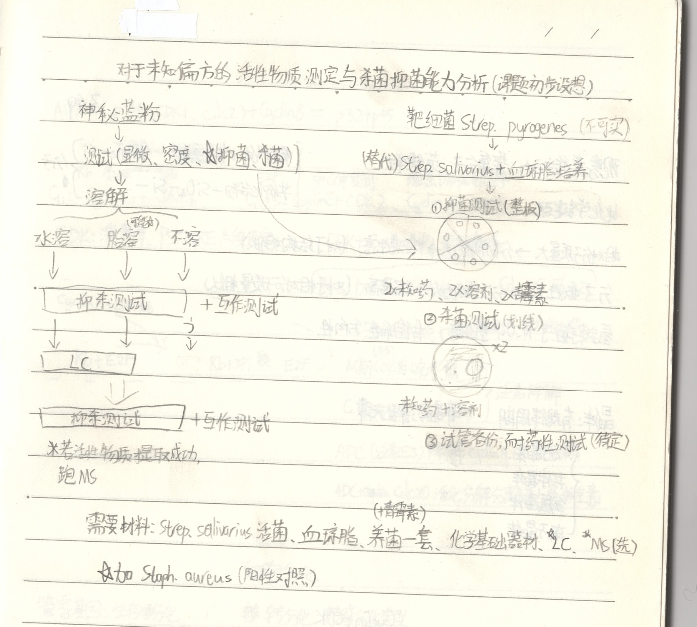
\includegraphics[width=0.8\textwidth]{figures/first_thoughts.png} 
    % \fbox{\begin{minipage}{0.8\textwidth}\centering 此处插入显微镜照片占位符 \end{minipage}}
    \caption{课题初步设想}
    \label{fig:first_thoughts}
\end{figure}

% 这里使用 longtable 制作跨页表格，防止日志太长被切断
\begin{longtable}{|c|c|p{3.5cm}|p{4.5cm}|p{3cm}|}
    \hline
    \textbf{日期} & \textbf{时间} & \textbf{操作/条件} & \textbf{现象/数据} & \textbf{备注} \\
    \hline
    \endfirsthead % 表格第一页的表头
    
    \hline
    \textbf{日期} & \textbf{时间} & \textbf{操作/条件} & \textbf{现象/数据} & \textbf{备注} \\
    \hline
    \endhead
    
    \hline
    \multicolumn{5}{|r|}{\textit{续下页...}} \\
    \endfoot
    
    \hline
    \endlastfoot % 表格最后一页的表尾

    % --- 日志内容开始 (直接复制修改这里) ---
    2023-10-01 & 09:00 & 配制 LB 培养基，灭菌 \SI{121}{\degreeCelsius} & 培养基澄清，无沉淀 & 批次 \#01 \\
    \hline
    2023-10-01 & 14:00 & 接种大肠杆菌，摇床培养 & 菌液略显浑浊 & 转速 \SI{200}{rpm} \\
    \hline
    2023-10-02 & 08:30 & 观察菌液浓度 (OD600) & OD 值 = 0.85 & 进入对数生长期 \\
    \hline
    2023-10-02 & 09:00 & 加入抑制剂 A (浓度 \SI{10}{mg/mL}) & 无明显变化 & 开始计时 \\
    \hline
    2023-10-02 & 12:00 & 取样涂布平板 & 菌落数量减少 & 见照片 Fig-A1 \\
    \hline

\end{longtable}

\section{附录：主要试剂配方}
\begin{itemize}
    \item \textbf{LB 培养基}: 胰蛋白胨 \SI{10}{g/L}, 酵母提取物 \SI{5}{g/L}, NaCl \SI{10}{g/L}.
    \item \textbf{缓冲液}: PBS (pH 7.4).
\end{itemize}

% ================= 附录结束 ================= % 引入外部文件，不需要写 .tex 后缀也可以，但写上更清晰

\end{document}